% DoseRAD2026 final submission — Task: PROTON-CT (single-task LNCS report, <=11 content pages).
\documentclass{llncs}
\usepackage{amsmath,amssymb,bm,mathtools}
\usepackage{graphicx,booktabs,array}
\usepackage[hidelinks]{hyperref}
\usepackage{tikz}
\usetikzlibrary{arrows.meta,positioning,fit,backgrounds}
\graphicspath{{figs/}}
\newcommand{\opS}{\mathcal{S}}\newcommand{\opD}{\mathcal{D}}\newcommand{\opX}{\mathcal{X}}
\newcommand{\opR}{\mathcal{R}}\newcommand{\opC}{\mathcal{C}}\newcommand{\gam}{\gamma}
\renewcommand{\topfraction}{.95}\renewcommand{\bottomfraction}{.6}
\renewcommand{\textfraction}{.05}\renewcommand{\floatpagefraction}{.75}
\setcounter{topnumber}{3}\setcounter{totalnumber}{5}

\begin{document}

\title{A Differentiable Pencil-Beam-Prior Residual 3D U-Net with a Batched GPU Engine for
Beamlet-Level Proton Dose Prediction on CT (DoseRAD2026 Proton-CT Task)}
\titlerunning{Pencil-Beam-Prior Residual U-Net for Proton-CT}
\author{Kai Wang \and Meixu Chen \and Rui Yang}
\authorrunning{K. Wang et al.}
\institute{Department of Radiation Oncology, University of Colorado Anschutz Medical Campus,
Aurora, CO, USA\\ \email{\{kai.2.wang,meixu.chen,ray.yang\}@cuanschutz.edu}}

\maketitle

\begin{abstract}
We predict the Monte-Carlo (MC) dose of every proton beamlet by correcting an analytical Hong
pencil-beam prior with a residual 3D U-Net. Five differentiable channels are computed per
beamlet from the CT-derived stopping power: density, skin-entry water-equivalent path length
(WEPL), the pencil-beam prior itself (ported to a self-contained GPU implementation,
$r{=}0.995$ against the pyRadPlan reference, so the deployed system computes its own prior with
no planning-system dependency), lateral distance, and energy. The prior supplies $\sim$95\% of
the dose; in ablation, correcting a systematic WEPL over-count adds $+2.4\,\gam$(1\%/1\,mm) and
the prior a further $+4.4$, lifting a plain U-Net from 89.2 to 97.0 on the development fold.
Under 5-fold cross-validation on the 75 public patients the model reaches plan
$\gam$1\%/1\,mm\,$=96.7\pm1.0$, the strongest of our four task systems. Deployment uses a
batched engine built on a geometric identity; pencil-beam-spot rays within one beam are exactly
parallel, so per-beam WEPL collapses to one orthographic beam's-eye-view cumulative sum
($388\times$ over ray-marching), with bucket-batched network forwards (exact by same-shape
bucketing) and streamed compressed output: 0.185\,s per dose map at unchanged gamma. On the
hidden preliminary test set the full-data submission scored $\gam$\,=\,95.60, per-beam MAE
0.0082, IDD 0.0047, stratified MAE 0.0077, DVH 0.83, well within the 500\,s gate.
\keywords{proton dose prediction \and pencil beam \and differentiable physics \and residual
learning \and WEPL}
\end{abstract}

\section{Introduction}
Proton dose calculation is dominated by range: the Bragg peak position is set by the integrated
stopping power along the beam path, so small upstream density errors displace large local doses.
Deep engines such as DoTA~\cite{dota} reach MC accuracy at millisecond latency but treat
transport as an implicit target. We factor the problem instead: an analytical, differentiable
physics operator $\opC$ turns the CT-derived density and the beamlet descriptor into dose-shaped
channels, including a full analytical pencil-beam prior~\cite{hong} that already supplies
$\sim$95\% of the answer; and a residual 3D U-Net $\opD_\theta$ corrects the remainder (lateral
penumbra, scatter tails, heterogeneity effects the pencil beam misses). Two properties of this
design matter in practice. First, data efficiency: with most of the dose supplied analytically,
the network learns a small, smooth correction, and 75 patients suffice for $\gam$1\%/1\,mm
$\approx97$. Second, deployability: we port the pencil-beam engine to a self-contained GPU
implementation, so the deployed container computes its own prior: no external
treatment-planning system at inference; and we exploit beam geometry to batch the entire
physics pipeline (Sec.~3.4). This report details the Proton-CT system; the same framework
serves our submissions to all four DoseRAD2026 tasks.

\begin{figure}[t]\centering
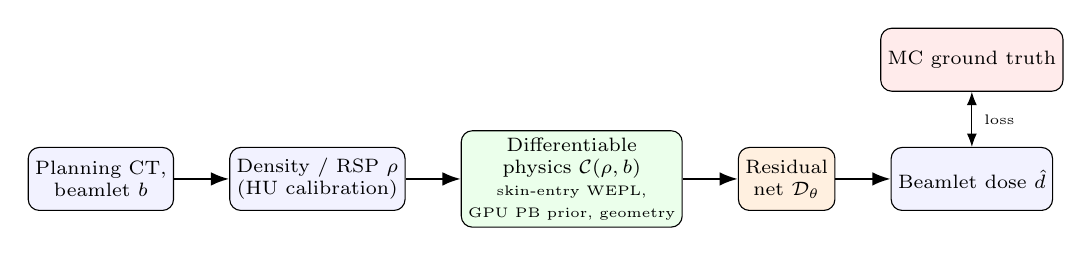
\begin{tikzpicture}[
 node distance=6mm and 7mm, >=Latex, font=\scriptsize,
 box/.style={draw, rounded corners, align=center, minimum height=8mm, inner sep=2.5pt, fill=blue!5},
 phys/.style={box, fill=green!8}, net/.style={box, fill=orange!12},
 every edge/.style={draw, ->, thick}]
\node[box] (img) {Planning CT,\\ beamlet $b$};
\node[box, right=of img] (dens) {Density / RSP $\rho$\\ (HU calibration)};
\node[phys, right=of dens] (chan) {Differentiable\\ physics $\opC(\rho,b)$\\ \tiny skin-entry WEPL,\\ \tiny GPU PB prior, geometry};
\node[net, right=of chan] (net) {Residual\\ net $\opD_\theta$};
\node[box, right=of net] (dose) {Beamlet dose $\hat d$};
\node[box, above=7mm of dose, fill=red!8] (mc) {MC ground truth};
\draw (img) edge (dens) (dens) edge (chan) (chan) edge (net) (net) edge (dose);
\draw[<->] (dose) -- (mc) node[midway,right=1pt]{\tiny loss};
\end{tikzpicture}
\caption{Proton-CT pipeline: per beamlet, differentiable channels (skin-entry WEPL, GPU
pencil-beam prior) from the CT stopping power; the U-Net learns the residual to
MC.}\label{fig:framework}
\end{figure}

\begin{figure}[t]\centering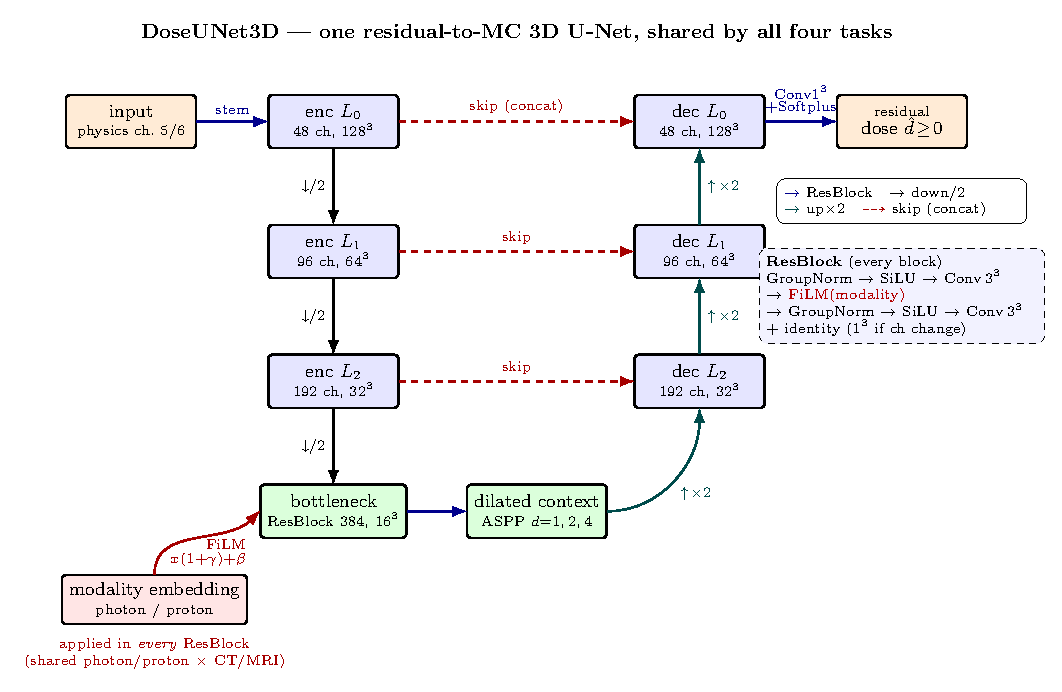
\includegraphics[width=.88\linewidth]{model_arch.pdf}
\caption{The dose network $\opD_\theta$ (DoseUNet3D): residual-to-MC 3D U-Net (channels
48/96/192/384), dilated-context (ASPP) bottleneck, Softplus head, FiLM modality conditioning in
every ResBlock; the photon and proton networks share this architecture but differ in input
channels.}\label{fig:arch}\end{figure}

\section{Methods}
\subsection{Data}
We use only the official DoseRAD2026 training set~\cite{challenge} (75 patients: 39 thorax, 36
abdomen; SynthRAD2025 cohort~\cite{synthrad}): per patient a planning CT, beam parameters, and
per-beamlet Monte-Carlo dose-to-medium in absolute Gy (Geant4 full particle transport; the treatment plans are generated with matRad~\cite{matrad}) on the native
$1{\times}1{\times}3$\,mm grid; several hundred to $\sim$a thousand beamlets (energy $\times$
spot) per patient. No external data are used for this task. Development used 5-fold
cross-validation over all 75 patients; \textbf{the final submitted model is retrained on all
75}, with the challenge leaderboard as the held-out validation signal.

\subsection{Model}
$\hat d=\opD_\theta(\opC(\rho,b))$ with $\rho$ treated as relative stopping power from the
official HU calibration. $\opC$ assembles \textbf{five differentiable channels} per beamlet:
(1) \emph{density/RSP} $\rho$;
(2) \emph{water-equivalent path length} (WEPL): a per-voxel integral of density from just
upstream of the skin to the voxel. WEPL is the single most range-determining input, and we
compute it with a corrected per-voxel scheme rather than a naive beam's-eye-view fan, which we
found to carry a systematic over-count worth $-2.4\,\gam$ (Table~\ref{tab:abl});
(3) the \emph{Hong pencil-beam prior}~\cite{hong}: the full analytical beamlet dose. We ported
the reference implementation (pyRadPlan) to a self-contained GPU version that reproduces it to
$r=0.995$ at $\sim$40\,ms/beamlet, and finetuned the residual network on this GPU prior so that
cached-prior training is identical to on-the-fly inference (train\,$=$\,deploy);
(4) \emph{lateral distance} from the beamlet axis (penumbra, multiple-Coulomb scatter);
(5) \emph{energy} (nominal Bragg-peak depth).
The per-ray \emph{skin-entry} rule applies to the WEPL and prior: depth accumulates only from
the first voxel with $\rho>0.05$\,g/cm$^3$; the prior is masked strictly upstream: no dose
before the body, internal cavities untouched. Figure~\ref{fig:chain} shows the deployed model's
complete residual-learning chain; note how small and structured the residual is once the
pencil-beam prior is subtracted.

\begin{figure}[t]\centering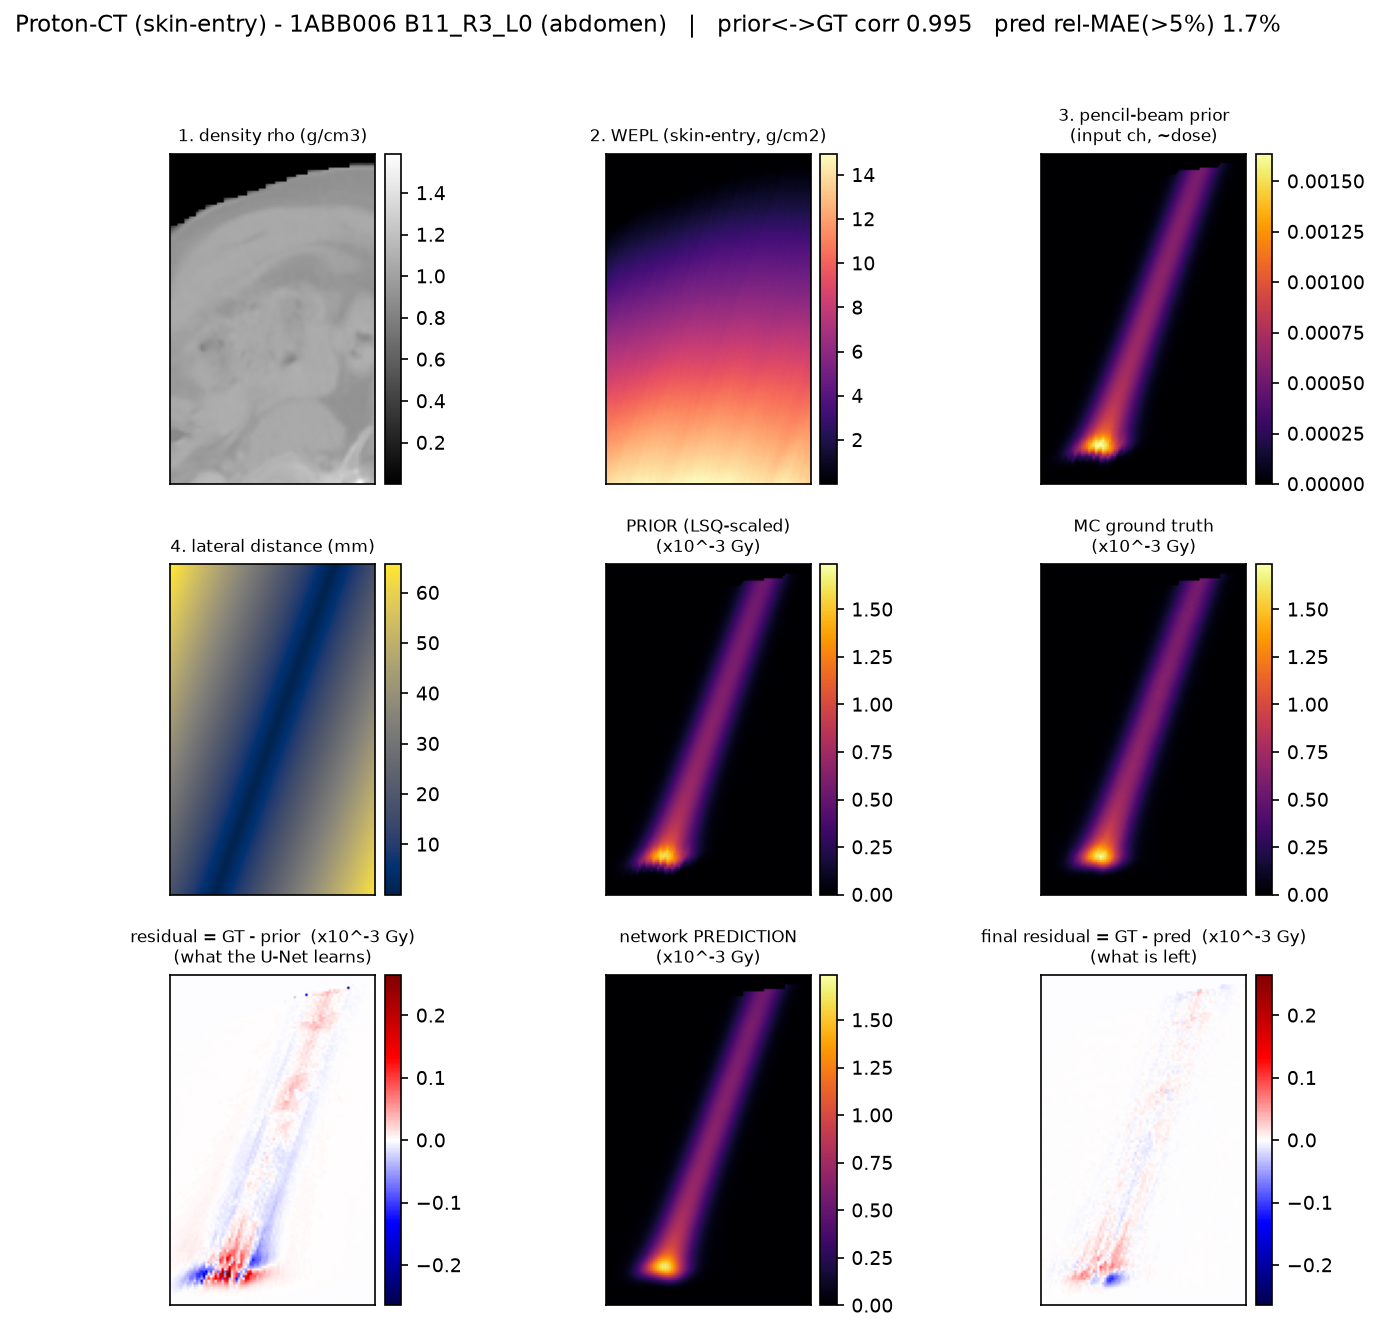
\includegraphics[width=.82\linewidth]{figS_residual_protonct_abdomen.png}
\caption{Residual-learning chain of the deployed skin-entry model (abdomen, peak-dose beamlet):
inputs (density/RSP, skin-entry WEPL, lateral distance) $\to$ GPU pencil-beam prior (already in
Gy, $\sim$95\% of the dose) $\to$ MC ground truth $\to$ residual (GT$-$prior) $\to$ prediction
$\to$ final residual (GT$-$pred); both residual panels share one symmetric
window.}\label{fig:chain}\end{figure}

\begin{figure}[t]\centering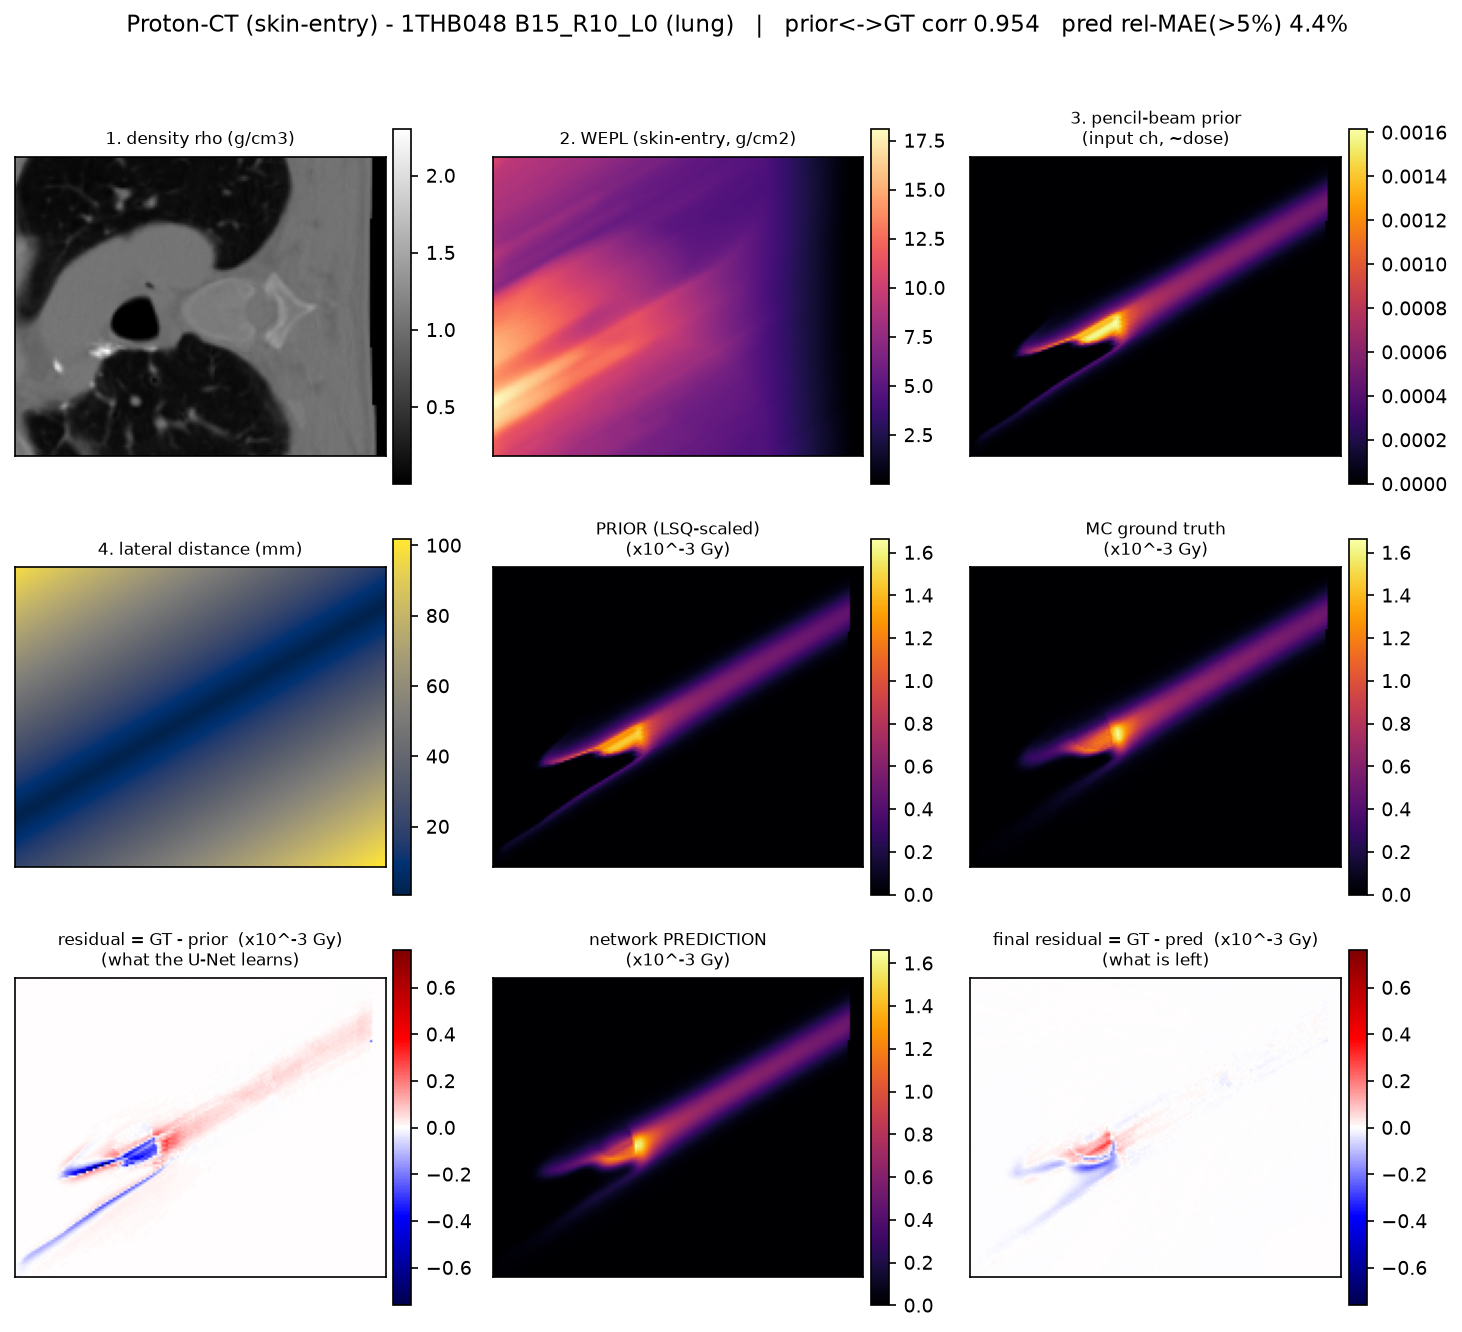
\includegraphics[width=.82\linewidth]{figS_residual_protonct_lung.png}
\caption{As Fig.~\ref{fig:chain}, lung case: the pencil-beam prior degrades most in low-density
lung (lateral heterogeneity), which is where the residual network
contributes.}\label{fig:chainlung}\end{figure}

\subsection{Training}
Loss: high-dose-weighted $L_1$ to MC (high-dose fraction 0.1, weight 10) plus bounded
penumbra/interface/lung terms; AdamW (lr $10^{-4}$ scratch, $2\times10^{-5}$ finetune), EMA,
gradient clipping; patches $32\times128^2$ (thin along the beam, wide laterally), batch 2--4.
The network trains $\sim$120k steps on cached channels, then a finetune on the GPU pencil-beam
prior (train\,$=$\,deploy) and a final convention-consistency finetune matching the deployed
batched WEPL engine (Sec.~3.4; the orthographic per-beam convention differs from the per-voxel
march by a mean $|\Delta\mathrm{WEPL}|$ of 0.18\,g/cm$^2$, and a short finetune makes the
network robust to both conventions). Reproducibility: fixed seeds, YAML configs, EMA
checkpoints; code and weights to be open-sourced (Sec.~6).

\subsection{Evaluation}
Internal: plan-level local $\gam$~\cite{gamma} (pymedphys, 1\%/1\,mm, $\ge$10\% Rx cutoff,
byte-identical to the vendored official code), per-beamlet masked MAE, official IDD and
stratified-MAE reimplementations, and a frozen 16-patient held-out cohort gating every
deployment change (\emph{no accuracy loss, no speed loss}). Runtime: official score
$T=t_{\rm fix}+N\cdot t_{\rm dose\,map}$, gate 500\,s/job, double-weighted; all engine work was
profiled at job scale under a strict 14.5\,GB platform memory budget (our development GPU has
32\,GB, which silently masks platform OOM; job-scale replicas at the platform budget caught two
such failures before submission).

\section{Results}
\subsection{Accuracy: cross-validated and hidden-test}
Per-fold CV $\gam$1/1: 96.7/97.7/96.9/94.9/97.5 (mean $\mathbf{96.7\pm1.0}$); the strongest of
our four task systems, reflecting the strength of the analytical prior. Development fold
($n=16$): $\gam$1/1 $=97.0\pm2.3$ (abdomen 98.2, lung 95.8), $\gam$3/3 $=99.9$; per-beamlet
masked MAE $0.89\pm0.22$\%. Table~\ref{tab:res} adds the official hidden-test metrics of the
full-data submission.

\begin{table}[t]\centering
\caption{Proton-CT results. CV: 5-fold over the 75 public patients. Hidden test: official
metrics of the final full-data submission on the preliminary test set (August 2026). Gate:
500\,s/job.}\label{tab:res}
\begin{tabular}{@{}lc@{}}\toprule
Metric & Value\\\midrule
CV plan $\gam$1\%/1\,mm (5-fold) & $96.7\pm1.0$\\
Hidden-test per-beam masked MAE & $0.0082\pm0.0025$\\
Hidden-test IDD curve distance & $0.0047\pm0.0025$\\
Hidden-test stratified plan MAE & $0.0077\pm0.0028$\\
Hidden-test plan $\gam$1\%/1\,mm & $95.60\pm3.33$\\
Hidden-test DVH clinical score & $0.83\pm0.35$\\
Hidden-test runtime per job & 191.7\,s (batched engine: 0.185\,s/map, 57\,s/309-map job)\\\bottomrule
\end{tabular}\end{table}

\subsection{Ablations: the prior does the heavy lifting}
Table~\ref{tab:abl} isolates the two Proton-CT-specific levers on the development fold. A plain
U-Net on uncorrected channels reaches 89.2; fixing the systematic WEPL over-count adds $+3.4$;
adding the pencil-beam prior a further $+3.1$; finetuning the residual on the deployable GPU
prior (train$=$deploy) closes the chain at 97.0. The analytical prior is not a warm start but
the backbone: it supplies $\sim$95\% of the dose, and the network's role is confined to the
residual the analytical model cannot express.

\begin{table}[h]\centering
\caption{Proton-CT ablation (plan $\gam$1\%/1\,mm, development fold, $n=16$).}\label{tab:abl}
\begin{tabular}{@{}lccc@{}}\toprule
configuration & ALL & abd & lung\\\midrule
no prior (WEPL uncorrected) & 89.2 & 90.7 & 87.6\\
no prior $+$ WEPL-fix & 92.6 & 93.1 & 92.2\\
$+$ pencil-beam prior & 95.7 & 96.9 & 94.5\\
$+$ GPU-PB finetune (train$=$deploy, deployed) & \textbf{97.0} & 98.2 & 95.8\\\bottomrule
\end{tabular}\end{table}

\subsection{Saturation: why extra training signals are flat here}
On the photon task, multi-modal joint training (one network over real- and synthetic-CT inputs)
gains $+2.8\,\gam$ cross-validated. The \emph{identical} experiment on Proton-CT is flat
($96.7\pm0.9$, mean per-fold change $-0.01$), and the real-CT-ceiling probe agrees ($-0.6$).
This is the expected behaviour of a residual architecture whose prior already supplies most of
the signal: the residual is small (penumbra and scatter tails) and the network operates near the
floor set by the prior's fidelity and label noise. The contrast with photons is a useful design
rule: \emph{invest extra training signal where the analytical prior is weak}.

\subsection{Error analysis: the lung deficit is a systematic over-prediction}
Aggregate gamma hides error structure, so we analyzed the failing voxels directly. In lung, the
failures are not symmetric noise: 73.7\% of gamma-failing voxels are \emph{over}-predictions
(binomial $p\approx3\times10^{-13}$ against symmetry); the model systematically deposits
slightly too much dose in low-density lung, plausibly inherited from the pencil-beam prior's
handling of lateral heterogeneity, which the residual network under-corrects. A post-hoc
lung-region deflation corrected the bias but degraded net lung gamma (the correction helps
failing voxels and harms passing ones), so the fix belongs in training, not post-processing; we
report the diagnosis as a target for the next iteration. Abdomen shows no such structure.


\begin{figure}[t]\centering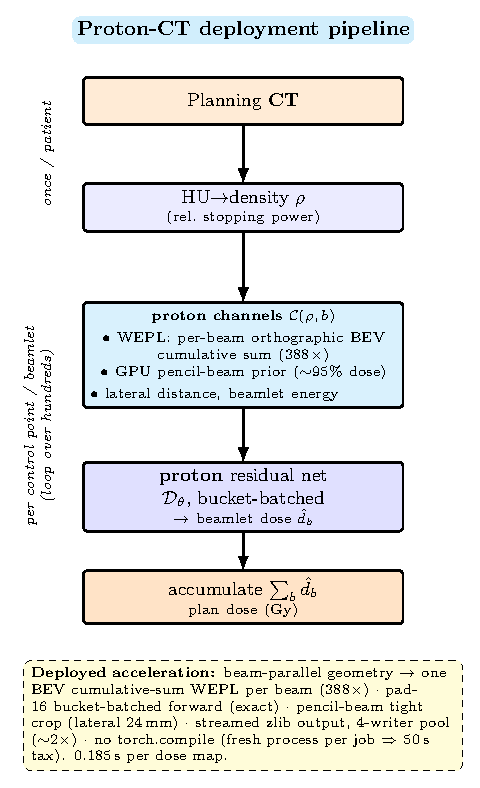
\includegraphics[width=.55\linewidth]{fig_deploy_protonct.pdf}
\caption{The deployed Proton-CT container: per patient, the density stage runs once; the
differentiable-channels $\to$ residual-net loop runs per control point/beamlet. The callout
lists the deployed acceleration measures and their measured effects.}\label{fig:deploy}\end{figure}

\subsection{Runtime engineering: a batched proton engine}
Proton jobs write one dose map per beamlet on the native $1{\times}1{\times}3$\,mm grid (tens
of GB per job) so both compute and write paths matter. Our engine (Table~\ref{tab:accel})
rests on a geometric identity: within one beam, pencil-beam-spot rays are \emph{exactly}
parallel (the virtual source translates with the spot), so the per-beam WEPL of all beamlets
collapses to a single orthographic beam's-eye-view cumulative sum; $388\times$ faster than
per-voxel ray-marching, and matched to training by the convention finetune of Sec.~2.3.
Downstream, beamlet crops are padded into shape buckets and batch-forwarded (plain GroupNorm is
per-sample, so same-shape bucketing keeps batching \emph{exact}; we abandoned a masked-GN
variant after it cost 13\,$\gam$), and finished frames stream through a 4-worker
zlib-compression pool that overlaps writing with GPU compute ($\sim$2$\times$ on the otherwise
write-bound path). End-to-end: 0.185\,s/map on the evaluation platform (57\,s for a 309-map
job), 1.7--2.0$\times$ over our previous per-beamlet engine at unchanged accuracy (held-out
$\gam$ 97.51 vs.\ 97.50). Two platform findings for future participants: (i) the evaluation
service starts a fresh process per job, so \texttt{torch.compile} pays its full $\sim$50\,s
compilation tax every job; at 250--310 maps/job the tax exceeds the $\sim$1.7$\times$
steady-state kernel gain, and multi-grid jobs recompile repeatedly (one measured job: 238\,s
compiled vs.\ 110\,s eager); our engine therefore ships \emph{without} compile; (ii)
per-beamlet crop tightening (lateral 24\,mm) is a free $1.2\times$ (91.5$\to$77\,ms/beamlet)
with gamma unchanged.

\emph{Memory engineering.} Two of our engine submissions failed on the platform with
out-of-memory errors that our 32\,GB development GPU had silently masked; the fixes; per-beam
chunked streaming (memory $O(\mathrm{chunk})$ instead of $O(\mathrm{plan})$), an explicit
batched-forward voxel cap tuned to the platform, and allocator
\texttt{expandable\_segments}; were validated by replaying the largest test-scale patients
under a hard 12.8\,GB cap before resubmission. We recommend this cap-replay protocol to any team
whose development hardware out-classes the evaluation instance.

\begin{table}[t]\centering
\caption{Proton-CT engine levers (all accuracy-gated; measured on the evaluation platform or
job-scale replicas at the 14.5\,GB platform memory budget).}\label{tab:accel}
\setlength{\tabcolsep}{4pt}\small
\begin{tabular}{@{}lll@{}}\toprule
Lever & Effect & Accuracy impact\\\midrule
Orthographic BEV cumulative-sum WEPL & $388\times$ WEPL build & convention finetune\\
Pad-16 bucketed batched forward & part of 1.7--2$\times$ e2e & exact (same-shape GN)\\
Pencil-beam tight crop (lateral 24\,mm) & 91.5$\to$77\,ms/beamlet & $\gam$ unchanged\\
Streamed zlib output, 4-writer pool & $\sim$2$\times$ (write-bound path) & lossless\\
Sub-cutoff quantisation of output & smaller writes & $\gam$ preserved (gated)\\
Batched engine, end-to-end & 0.307$\to$0.185\,s/map & held-out 97.51 vs.\ 97.50\\
\emph{Rejected:} \texttt{torch.compile} & $+50$\,s/job tax, recompile storms & --- \\\bottomrule
\end{tabular}\end{table}



\begin{figure}[t]\centering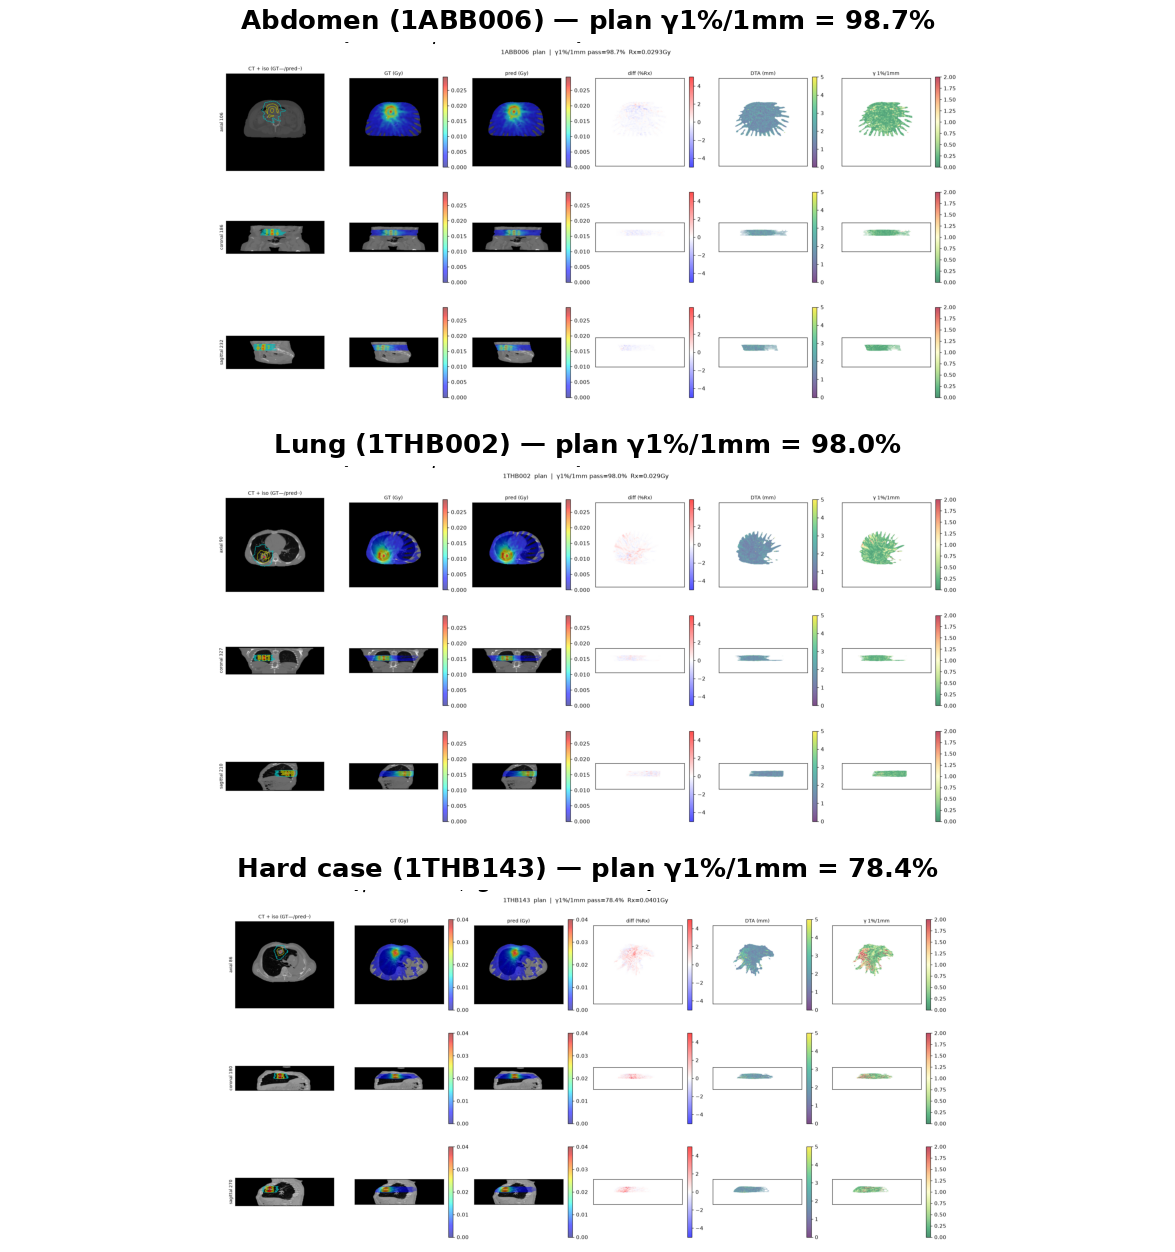
\includegraphics[width=.92\linewidth]{fig_qual_protonct.png}
\caption{Qualitative Proton-CT results on three cases spanning the difficulty range: abdomen (1ABB006, plan $\gam$1/1 $=98.7$), lung (1THB002, $98.0$), and the geometrically hard case 1THB143 ($78.4$; the worst patient in all four challenge tasks simultaneously, yet largely passing at 3\%/3\,mm: small-magnitude errors at steep lung--tissue interfaces). Columns: image with GT (solid) and predicted (dashed) isodose, MC dose, predicted dose, difference, distance-to-agreement, local $\gam$1\%/1\,mm.}\label{fig:qual}\end{figure}

\section{Discussion}
Proton-CT is the clearest demonstration of the physics-prior residual design: the analytical
pencil beam supplies $\sim$95\% of the dose, the U-Net corrects only what the analytical model
cannot express, and the result ($96.7\pm1.0$ cross-validated) is our strongest task system with
the least data hunger. The deployable GPU port of the prior removes the planning-system
dependency that keeps many published engines from running standalone, and the batched engine
shows that careful use of beam geometry buys $\sim$2$\times$ wall-clock at exactly zero accuracy
cost. \textbf{Limitations and generalizability.} Single benchmark (abdomen/thorax), one machine
model; the analytical prior assumes the machine's beam model, so transferring to another machine
requires re-fitting the prior (the network, learning only a residual, should transfer more
easily). Ablation deltas are single-fold ($n=16$); headline accuracy is the 5-fold CV. Lung
remains the harder site (95.8 vs.\ 98.2): the pencil beam handles lateral heterogeneity worst
exactly there.

\textbf{Future work.} (i) \emph{Fix the lung over-prediction at the source}: our error analysis
(Sec.~3.4) localizes a systematic bias that post-processing cannot remove; a lung-aware loss
asymmetry or a heterogeneity-corrected prior variant (e.g.\ subdividing the pencil beam
laterally in low-density regions) is the natural next training-side intervention. (ii)
\emph{Machine transfer}: the residual design should transfer across machines by re-fitting only
the analytical prior; validating this on a second beam model would substantiate the framework's
main practical claim. (iii) \emph{DVH-aware selection}: as on the photon task, our DVH clinical
score lags our gamma rank; internalizing the official DVH pipeline for checkpoint selection is
cheap and likely valuable. (iv) \emph{Gradient-based planning}: the engine is differentiable
down to beamlet weights and energies, making it a candidate physics layer for direct proton
spot-map optimization~\cite{pydosert,achlatis}; with the batched engine at 0.185\,s/map, an
optimization loop over a full spot map is already interactive-rate.

\section{Author Contributions (CRediT)}
\textbf{Kai Wang:} Conceptualization, Methodology, Software, Validation, Formal analysis,
Investigation, Data curation, Writing -- original draft, Visualization.
\textbf{Meixu Chen:} Software (deployment and runtime optimization), Investigation
(acceleration study), Validation, Writing -- review \& editing.
\textbf{Rui Yang:} Conceptualization, Methodology, Writing -- review \& editing, Supervision.

\section{Other Information}
\textbf{Funding:} No external funding was received for this work.
\textbf{Collaborators:} None beyond the listed authors.
\textbf{Writing assistance:} Large-language-model assistance (Claude, Anthropic) was used in drafting and editing the text of this report; all methods, experiments, analyses and conclusions are the authors' own.
\textbf{Code availability:} The full implementation (models, differentiable physics operators,
the GPU pencil-beam prior, deployment containers, and weights) will be released open-source at
\url{https://github.com/wangkaiwan/PhyPriorNet} before the challenge deadline (2026-10-01).

\clearpage
\begin{thebibliography}{9}\small
\bibitem{dota} Pastor-Serrano, O., Perk\'o, Z.: Millisecond speed deep learning based proton dose
calculation with Monte Carlo accuracy. Phys. Med. Biol. \textbf{67}, 105006 (2022)
\bibitem{hong} Hong, L., et al.: A pencil beam algorithm for proton dose calculations. Phys. Med.
Biol. \textbf{41}, 1305--1330 (1996)
\bibitem{matrad} Wieser, H.P., et al.: Development of the open-source dose calculation and
optimization toolkit matRad. Med. Phys. \textbf{44}, 2556--2568 (2017)
\bibitem{gamma} Low, D.A., Harms, W.B., Mutic, S., Purdy, J.A.: A technique for the quantitative
evaluation of dose distributions. Med. Phys. \textbf{25}, 656--661 (1998)
\bibitem{challenge} DoseRAD2026 Grand Challenge, \url{https://doserad2026.grand-challenge.org} (2026)
\bibitem{synthrad} Thummerer, A., et al.: SynthRAD2025 Grand Challenge dataset: generating
synthetic CTs for radiotherapy. Med. Phys. (2025)
\bibitem{pydosert} Simk\'o, A., et al.: A physics-informed, plug-and-play dose engine for
gradient-based radiotherapy treatment planning. arXiv:2512.18863 (2025)
\bibitem{achlatis} Achlatis, S., Gavves, E., Sonke, J.-J.: Physics-guided radiotherapy treatment
planning with deep learning. arXiv:2506.19880 (2025)
\end{thebibliography}

\end{document}
